%% LyX 1.5.5 created this file.  For more info, see http://www.lyx.org/.
%% Do not edit unless you really know what you are doing.
\documentclass[a4paper,czech,czech,openright,cleardoubleempty,BCOR10mm,DIV11]{scrreprt}
\usepackage[T1]{fontenc}
\usepackage[utf8]{inputenc}
\usepackage{array}
\usepackage{longtable}
\usepackage{varioref}
\usepackage{wrapfig}
\usepackage{fancybox}
\usepackage{calc}
\usepackage{framed}
\usepackage{url}
\usepackage{graphicx}
\usepackage{color}
\usepackage{float}
\usepackage{svg}
\usepackage{amsmath}
\usepackage{makecell}
\usepackage{fourier} 
\usepackage{pdfpages}

\makeatletter

%%%%%%%%%%%%%%%%%%%%%%%%%%%%%% LyX specific LaTeX coěmmands.
\providecommand{\LyX}{L\kern-.1667em\lower.25em\hbox{Y}\kern-.125emX\@}
\newcommand{\lyxline}[1][1pt]{%
  \par\noindent%
  \rule[.5ex]{\linewidth}{#1}\par}
\newcommand{\noun}[1]{\textsc{#1}}
%% Special footnote code from the package 'stblftnt.sty'
%% Author: Robin Fairbairns -- Last revised Dec 13 1996
\let\SF@@footnote\footnote
\def\footnote{\ifx\protect\@typeset@protect
    \expandafter\SF@@footnote
  \else
    \expandafter\SF@gobble@opt
  \fi
}

\expandafter\def\csname SF@gobble@opt \endcsname{\@ifnextchar[%]
  \SF@gobble@twobracket
  \@gobble
}
\edef\SF@gobble@opt{\noexpand\protect
  \expandafter\noexpand\csname SF@gobble@opt \endcsname}
\def\SF@gobble@twobracket[#1]#2{}
%% Because html converters don't know tabularnewline
\providecommand{\tabularnewline}{\\}

%%%%%%%%%%%%%%%%%%%%%%%%%%%%%% Textclass specific LaTeX commands.
\newenvironment{lyxcode}
{\begin{list}{}{
\setlength{\rightmargin}{\leftmargin}
\setlength{\listparindent}{0pt}% needed for AMS classes
\raggedright
\setlength{\itemsep}{0pt}
\setlength{\parsep}{0pt}
\normalfont\ttfamily}%
 \item[]}
{\end{list}}

%%%%%%%%%%%%%%%%%%%%%%%%%%%%%% User specified LaTeX commands.
%<-------------------------------společná nastavení------------------------------>
\usepackage[czech]{babel}%počeštění názvů (Obsah, Kapitola, Literatura atp.)
\usepackage[]{hyperref} %odkazy v  pdf jsou klikací s barevnými rámečky
\usepackage[numbers,sort&compress]{natbib} %balíček pro citace literatury  
\usepackage{hypernat}%interakce mezi hyperref a natbib
\newcommand{\BibTeX}{{\sc Bib}\TeX}%BibTeX logo
\hypersetup{   % Nastavení polí PDF dokumentu 
pdftitle={Evaluation of Container-based Virtualization for standard company environment},%   
pdfauthor={Pavel Cizinsky},%  
pdfsubject={},%   
pdfkeywords={Docker, Kubernetes, Kotejner, Virtualizace}%                             
}
\usepackage{multicol}




%<-----------------------------volání stylů----------------------------------------->
% (znak % je označení komentáře: co je za ním, není aktivní)
%<------------------------------------písmo----------------------------------------->
%\usepackage{packages/bc-latinmodern}
%\usepackage{packages/bc-times}
\usepackage{packages/bc-palatino}
%\usepackage{packages/bc-iwona}
%\usepackage{packages/bc-helvetika}


%<------------------------------záhlaví stránek------------------------------------>
%\usepackage{packages/bc-headings}
\usepackage{packages/bc-fancyhdr}

%<------------------------------hlavičky kapitol------------------------------------>
%\usepackage{packages/bc-neueskapitel}
%\usepackage{packages/bc-fancychap}

\makeatother

\usepackage{babel}

%java code block%

\usepackage{listings}
\usepackage{color}

\definecolor{dkgreen}{rgb}{0,0.6,0}
\definecolor{gray}{rgb}{0.5,0.5,0.5}
\definecolor{mauve}{rgb}{0.58,0,0.82}

% syntax highlight pro jazyk Javascript %
\definecolor{purple}{rgb}{0.65, 0.12, 0.82}
\lstdefinelanguage{JavaScript}{
  keywords={break, case, catch, const, continue, debugger, default, delete, do, else, false, finally, for, function, if, in, instanceof, let, new, null, return, switch, static, this, throw, true, try, typeof, var, void, while, with},
  morecomment=[l]{//},
  morecomment=[s]{/*}{*/},
  morestring=[b]',
  morestring=[b]",
  ndkeywords={class, constructor, export, extends, boolean, throw, implements, import},
  keywordstyle=\color{blue}\bfseries,
  ndkeywordstyle=\color{gray}\bfseries,
  identifierstyle=\color{black},
  commentstyle=\color{purple}\ttfamily,
  stringstyle=\color{red}\ttfamily,
  sensitive=true
}

\lstset{,
  language=Javascript,
  aboveskip=3mm,
  belowskip=3mm,
  showstringspaces=false,
  columns=flexible,
  inputencoding=utf8,
    extendedchars=true,
    literate=%
    {á}{{\'a}}1
    {č}{{\v{c}}}1
    {ď}{{\v{d}}}1
    {é}{{\'e}}1
    {ě}{{\v{e}}}1
    {í}{{\'i}}1
    {ň}{{\v{n}}}1
    {ó}{{\'o}}1
    {ř}{{\v{r}}}1
    {š}{{\v{s}}}1
    {ť}{{\v{t}}}1
    {ú}{{\'u}}1
    {ů}{{\r{u}}}1
    {ý}{{\'y}}1
    {ž}{{\v{z}}}1
    {Á}{{\'A}}1
    {Č}{{\v{C}}}1
    {Ď}{{\v{D}}}1
    {É}{{\'E}}1
    {Ě}{{\v{E}}}1
    {Í}{{\'I}}1
    {Ň}{{\v{N}}}1
    {Ó}{{\'O}}1
    {Ř}{{\v{R}}}1
    {Š}{{\v{S}}}1
    {Ť}{{\v{T}}}1
    {Ú}{{\'U}}1
    {Ů}{{\r{U}}}1
    {Ý}{{\'Y}}1
    {Ž}{{\v{Z}}}1,
  basicstyle={\small\ttfamily},
  xleftmargin=1cm,
  keywordstyle=\color{blue},
  commentstyle=\color{dkgreen},
  stringstyle=\color{mauve},
  breaklines=true,
  breakatwhitespace=true,
  tabsize=3
}
\usepackage{url}
\makeatletter
\g@addto@macro{\UrlBreaks}{\UrlOrds}
\makeatother

% vlastni package
\usepackage{placeins}
\usepackage{multirow}
\usepackage{pdfpages}
% fonty popisku
\usepackage[font=small,labelfont=bf]{caption}
% radkovani 
\renewcommand{\baselinestretch}{1.2}
\renewcommand*{\lstlistingname}{Kód} %prejmenovani lstlisting
\renewcommand*{\lstlistlistingname}{Seznam ukázek kódu}
% vlastni styly tabulek
\newcolumntype{C}[1]{>{\centering\arraybackslash}m{#1}}
\begin{document}

\cleardoublepage{}~\thispagestyle{empty}\begin{center}\pagenumbering{roman}\vspace{10mm}


\textsf{\textsc{\noun{\LARGE Univerzita Hradec Králové}}}\\
\vspace{0.5em}
\textsc{\noun{\LARGE Fakulta informatiky a managementu}}\\
\vspace*{1em}
\textsf{\textsc{\noun{\Large katedra informačních technologií }}}


%%% Aby vložení loga  správně fungovalo, je třeba mít soubor uhk.png nahraný v adresáři logo,
%%% tj. v adresáři, kde se nachází překládaný zdrojový soubor. 
\vspace{4cm}

\textsf{\huge BAKALÁŘSKÁ PRÁCE}{\huge \par}

\vspace{15mm}


\textsf{\LARGE Využití kontejnerové virtualizace pro standardní firemní prostředí}{\LARGE \par}

\vspace{10mm}


\end{center} 

\vspace*{\fill}


\vspace{10mm}


\begin{description}
%studijni obor???
\item [{{\large Autor:}}] \noindent \textsf{\large Pavel Čižinský}{\large \par}
\item [{{\large Studijní obor:}}] \noindent \textsf{\large Aplikovaná informatika}{\large \par}
\item [{{\large Vedoucí~práce:}}] \noindent \textsf{\large Ing. Jakub Pavlík, MSc.}{\large \hfill{}}\textsf{\large Hradec Králové, 2017}{\large{}
% doplňte rok vzniku vaší bakalářské práce
}{\large \par}
\end{description}

\clearpage{}
~\thispagestyle{empty}{\small ~\vfill{}
}{\small \par}

\noindent {\small \vfill{}
 % nastavuje dynamické umístění následujícího textu do spodní části stránky
~}{\small \par}

\noindent {\small Prohlašuji, že jsem bakalářskou práci vypracoval samostatně a uvedl jsem všechny použité prameny a literaturu.}{\small \par}

{\small \bigskip{}
}\noindent {\small{} V Jaroměři dne \today\hspace{\fill}Pavel Čižinský}\\
{\small{} % doplňte patřičné datum, jméno a příjmení
}{\small \par}

{\small %%%   Výtisk pak na tomto míste nezapomeňte PODEPSAT!
%%%                                         *********
}{\small \par}

\clearpage{}
~\thispagestyle{empty}{\small ~\vfill{}
}{\small \par}

\noindent {\small Rád bych poděkoval Ing. Jakubu Pavlíkovi, MSc. za odborné vedení práce, podnětné rady a čas, který mi věnoval. \newpage{}}{\small \par}
\clearpage{}
~\thispagestyle{empty}{\small ~\vfill{}
}{\small \par}
\noindent {\small \vfill{}
 % nastavuje dynamické umístění následujícího textu do spodní části stránky
~}{\small \par}
\section*{Anotace}
Tato bakalářská práce pojednává o kontejnerové virtualizaci, zabývá se problematikou nasazení kontejnerů do standardního firemního prostředí. První část je věnována představení virtualizace obecně a její porovnání s kontejnerovou virtualizací. Následně je řešena problematika orchestrace a ovládání kontejnerového prostředí. Čtvrtá a pátá kapitola je věnována analýze a převodu aplikace do kontejnerů, součástí  kapitoly pět je praktická ukázka funkčnosti orchestrátoru. Cílem této práce je seznámení čtenáře s konceptem kontejnerů a zjistit jejich využitelnost v produkčním prostředí a možnost převodu klasické aplikace do kontejnerů.
\subsubsection*{Klíčová slova}
Docker, Kubernetes, Cluster, Kontejnery, Virtualizace

\section*{Annotation}
Title: Evaluation of Container-based Virtualization for standard company environment
\vspace{0.5cm}\FloatBarrier
This Bachelor’s thesis describes container-based virtualization especially the issues in its use in standard company environment. The first part is dedicated to intruducing general virtualization and its comparison to container-based virtualization. Afterward is tackled the troubleshooting of orchestration and control of the container-based environment.
The fourth and fifth chapters are devoted to the analysis and conversion of application into containers. Practical example of the orchestration's functionality is included in chapter five.
The aim of this work is to familiarize the reader with the concept of containers and to find out their applicability in the production environment as well as the ability to convert a classic application into containers.

\subsubsection*{Key words}
Docker, Kubernetes, Cluster, Containers, Virtualization

\noindent {\small ~\vfill{}
}{\small \par}

\cleardoublepage{}\thispagestyle{empty}{\small \tableofcontents{}% vkládá automaticky generovaný obsah dokumentu
\cleardoublepage{}}{\small \par}

\include{tex/chap01}
\include{tex/chap02}
\include{tex/chap03}
\include{tex/chap04}
\include{tex/chap05}
\include{tex/chap06}

\addcontentsline{toc}{chapter}{Literatura} 

\begin{thebibliography}{10}
	
\end{thebibliography}


\cleardoublepage{}

%\include{tex/prilohy}
\appendix
\pagenumbering{Roman}

\chapter{Cizí výrazy}
\begin{itemize}
\end{itemize}

\listoffigures
\listoftables
\lstlistoflistings

%zadani
%\includepdf[pages={1},scale=0.8]{zadani2}
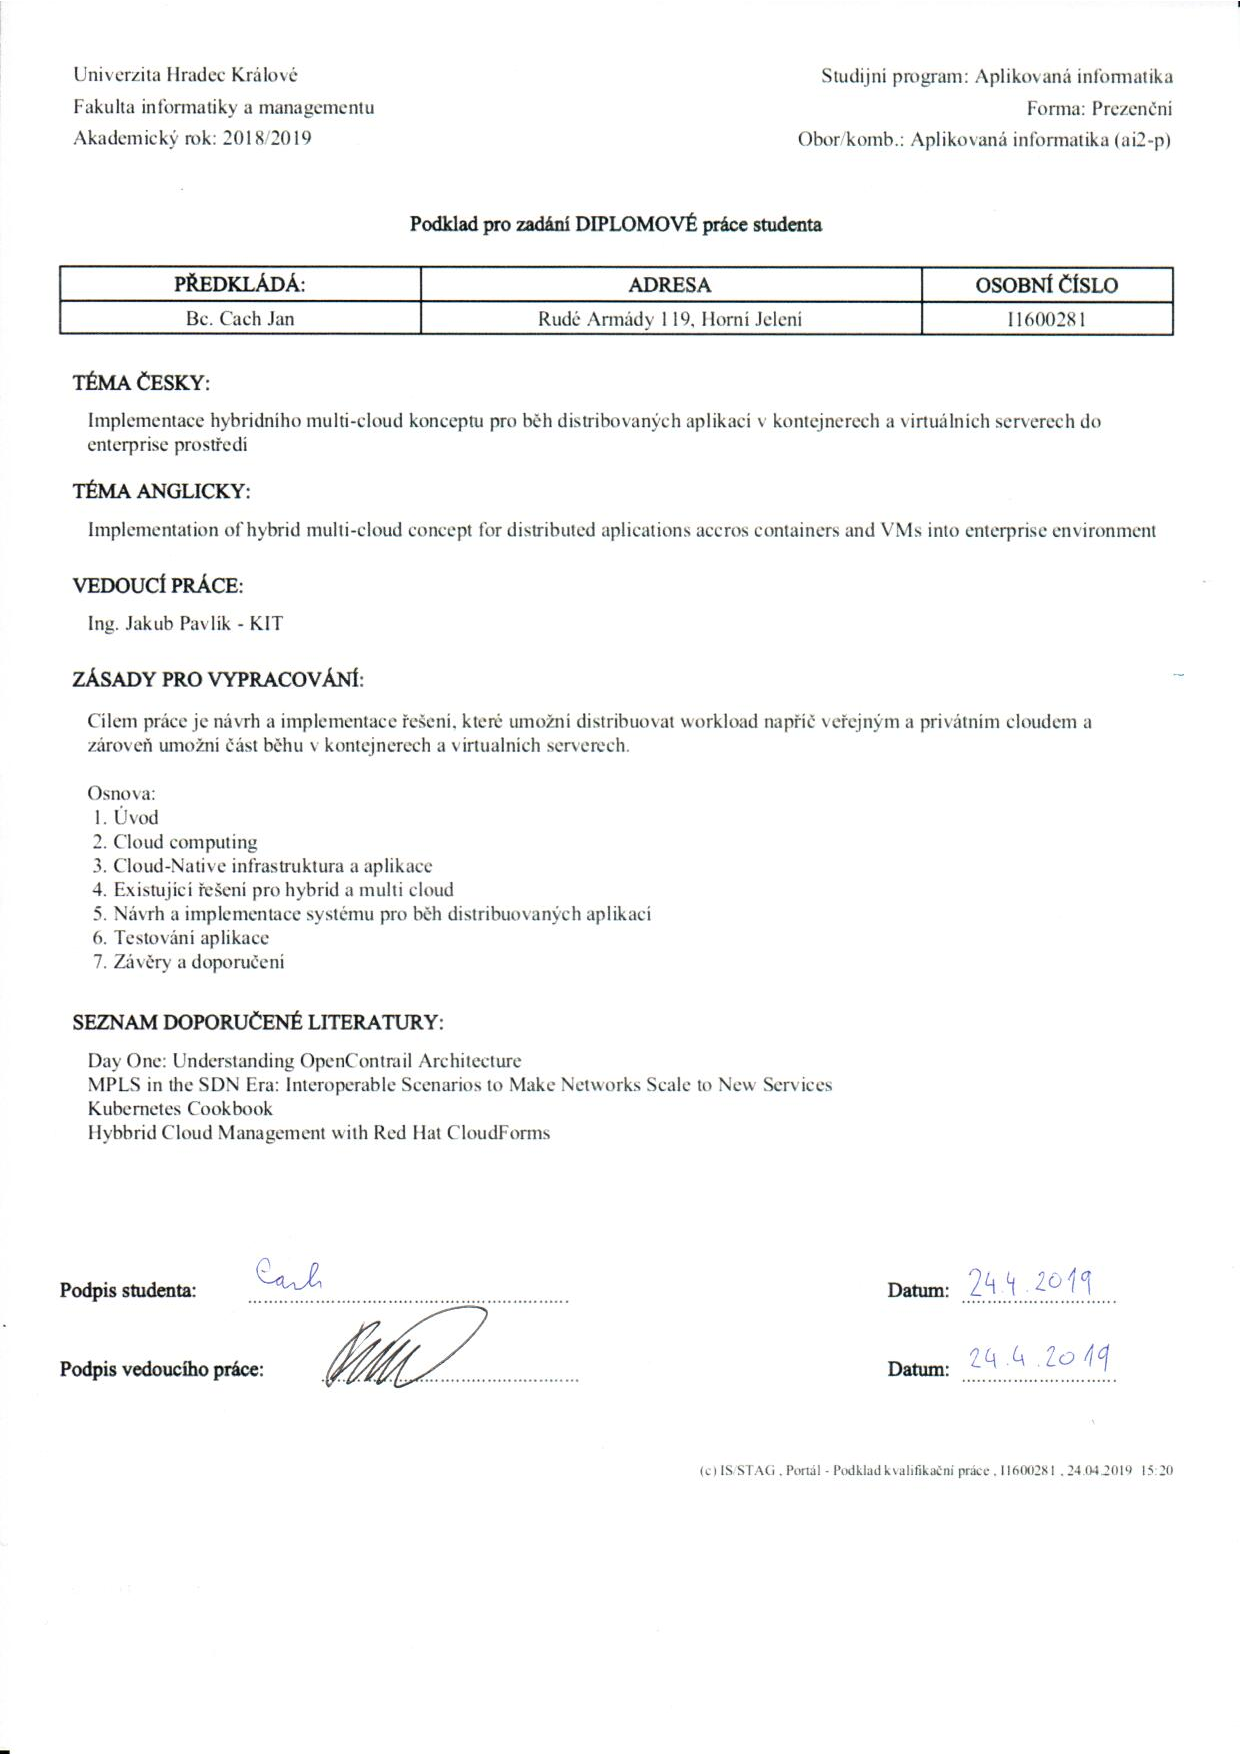
\includepdf[pages={1}]{zadani.pdf}

\clearpage{}
\end{document}
